\documentclass[oneside,a4paper,14pt]{extarticle}
\usepackage[a4paper,letterpaper,top=20mm,bottom=20mm,left=20mm,right=10mm]{geometry}
\usepackage[russian]{babel}
\usepackage{indentfirst}
\usepackage{graphicx}
\usepackage{caption}
\usepackage{titlesec}
\usepackage{minted, fancyvrb}
\usepackage{hyperref}
\usepackage{enumitem}
\usepackage{amsmath}
\usepackage{fancyhdr}
\usepackage{colortbl}
\usepackage[dvipsnames]{xcolor}
\usepackage{float}
\usepackage{tikz-timing}
\usepackage{tikz}
\usetikzlibrary{karnaugh}

% Настройка автоматических подписей к рисункам (Замена Рис. на Рисунок и тире в качестве разделителя)
\DeclareCaptionLabelSeparator{customdash}{~---~}
\captionsetup[figure]{name=Рисунок, labelsep=customdash, justification=centering}

\setminted{style = rainbow_dash, fontsize = \small}

% Форматирование заголовков
\titleformat{\section}{\normalsize\bfseries}{\thesection}{1em}{}
\titleformat{\subsection}{\normalsize\bfseries}{\thesubsection}{1em}{}
\titleformat{\subsubsection}{\normalsize\bfseries}{\thesubsubsection}{1em}{}

% Интерлиньяж и абзац
\renewcommand\baselinestretch{1.33}
\setlength{\parindent}{1.25cm}

% Для всех списков
\setlist[enumerate]{
  left=0.5\parindent,
  label=\arabic*.,
  itemsep=0pt,
  topsep=5pt,
  partopsep=0pt,
  parsep=0pt
}
\setlist[itemize]{
  left=0.5\parindent,
  itemsep=0pt,
  topsep=5pt,
  partopsep=0pt,
  parsep=0pt
}

% Гиперссылки
\hypersetup{
  colorlinks=true,
  linkcolor=black,
  urlcolor=blue,
  pdfborder={0 0 0},
  pdftitle={Контрольная работа: Построение 7-битного счётчика с переменным коэффициентом пересчёта},
  pdfauthor={Черкасов А.А.},
}

\begin{document}

\newpage
\thispagestyle{empty}
\begin{center}
  МИНИСТЕРСТВО НАУКИ И ВЫСШЕГО ОБРАЗОВАНИЯ РОССИЙСКОЙ ФЕДЕРАЦИИ\\
  ФЕДЕРАЛЬНОЕ ГОСУДАРСТВЕННОЕ БЮДЖЕТНОЕ УЧРЕЖДЕНИЕ ВЫСШЕГО ОБРАЗОВАНИЯ\\
  <<ВЯТСКИЙ ГОСУДАРСТВЕННЫЙ УНИВЕРСИТЕТ>>\\
  Институт математики и информационных систем\\
  Факультет автоматики и вычислительной техники\\
  Кафедра электронных вычислительных машин
\end{center}
\vspace{10mm}

\hfill
\begin{tabular}{l}
  \footnotesize Дата сдачи на проверку:                                          \\
  \footnotesize <<\rule[-1mm]{5mm}{0.10mm}\/>>\rule[-1mm]{20mm}{0.10mm}\ 2026 г. \\
  \footnotesize Проверено:                                                       \\
  \footnotesize <<\rule[-1mm]{5mm}{0.10mm}\/>>\rule[-1mm]{20mm}{0.10mm}\ 2026 г. \\
\end{tabular}
\vfill

\begin{center}
  Отчёт по контрольной работе\\
  по теме\\
  <<Построение 7-битного счётчика с переменным коэффициентом пересчёта>>\\
  по дисциплине\\
  <<Цифровая схемотехника>>\\
\end{center}
\vspace{25mm}
\noindent
\begin{tabular}{ll}
  Разработали студенты гр. ИВТб-2301-05-00 & \hspace{5mm}\rule[-1mm]{30mm}{0.10mm}\,/Черкасов А. А./ \\
                                           & \hspace{12.5mm}\footnotesize(подпись)                   \\
  Преподаватель                            & \hspace{5mm}\rule[-1mm]{30mm}{0.10mm}\,/Мельцов В. Ю./  \\
                                           & \hspace{12.5mm}\footnotesize(подпись)                   \\
\end{tabular}

\noindent
\begin{tabular}{lp{58mm}r}
  Работа защищена &  & \hspace{5mm}<<\rule[-1mm]{5mm}{0.10mm}\/>>\rule[-1mm]{30mm}{0.10mm}\ 2026 г.
\end{tabular}
\vfill

\begin{center}
  Киров\\
  2026
\end{center}

\newpage\thispagestyle{plain}

\section{Цель работы}
Получить теоретические и практические навыки проектирования и расчета последовательностных цифровых устройств со сложной внутренней структурой. Синтезировать функциональную и принципиальную схемы 7-битного двоичного счётчика с заданным коэффициентом пересчёта 103 на базе стандартных интегральных микросхем ТТЛ-логики.

\section{Теоретическое описание}
\subsection{Двоичный счётчик ИЕ7}
Интегральная микросхема К155ИЕ7 представляет собой 4-разрядный реверсивный синхронный двоичный счётчик с возможностью асинхронной параллельной предварительной установки данных. Компонент снабжён информационными входами предустановки $D_0\dots D_3$, тактовыми входами прямого и обратного счёта, асинхронным входом сброса $R$, входом разрешения параллельной записи $WR$ и разрядными выходами $Q_0\dots Q_3$. Изменение внутренних состояний автомата памяти происходит по спаду тактового импульса на соответствующем счётном входе.

\subsection{Программируемый коэффициент пересчёта}
Для реализации произвольного или укороченного коэффициента деления (пересчёта) используется метод динамической параллельной загрузки (parallel load) начального кода при достижении граничного состояния. Каскадное последовательное включение двух микросхем ИЕ7 формирует единую 8-битную структуру, из которой для решения поставленной задачи задействуется 7 разрядов. 

При регистрации выходного кодового слова, соответствующего эквиваленту коэффициента 103, внешняя комбинационная логика на базе ИС ЛА3, ЛА4 и ЛН1 генерирует результирующий импульс управления, поступающий на входы разрешения записи $WR$. Данный сигнал инициирует принудительный занос опорной кодовой комбинации, после чего цикл функционирования периодически повторяется, обеспечивая коэффициент пересчёта, равный 103.

\subsection{D-триггер ТМ2}
Микросхема К155ТМ2 содержит два независимых синхронных D-триггера с прямыми и инверсными управляющими входами асинхронной установки. В спроектированном устройстве один из триггеров задействуется в цепи обратной связи для временного выравнивания, устранения эффекта <<гонок>> сигналов в комбинационной логике дешифратора граничного кода и формирования стабильного выходного стробирующего импульса.

\section{Функциональная схема счётчика}
На основании алгоритма переходов разработана функциональная схема 7-битного счётчика с коэффициентом пересчёта 103. Каскадирование двух ИС ИЕ7 выполнено путём коммутации выходов переноса старшего и младшего разрядов. Обратная связь, обеспечивающая циклическое деление частоты, реализована на логических элементах серий ЛА3 и ЛА4.

\begin{figure}[H]
  \centering
  
\includegraphics[width=0.9\textwidth]{pics/functional_diagram.png}
  \caption{Функциональная схема 7-битного счётчика с коэффициентом пересчёта 103}
\end{figure}

\section{Принципиальная схема устройства}
Схема электрическая принципиальная устройства разработана в элементном базисе транзисторно-транзисторной логики (ТТЛ). Спецификация проекта включает интегральные микросхемы: \textbf{ЛА3} (четыре элемента 2И-НЕ), \textbf{ЛА4} (три элемента 3И-НЕ), \textbf{ЛН1} (шесть инверторов НЕ), \textbf{ИЕ7} (два 4-разрядных двоичных счётчика) и \textbf{ТМ2} (двухступенчатый D-триггер). Электрические связи и цоколёвка корпусов соответствуют паспортным техническим характеристикам компонентов. Номинальное напряжение шины питания составляет $+5$~В.

\begin{figure}[H]
  \centering
  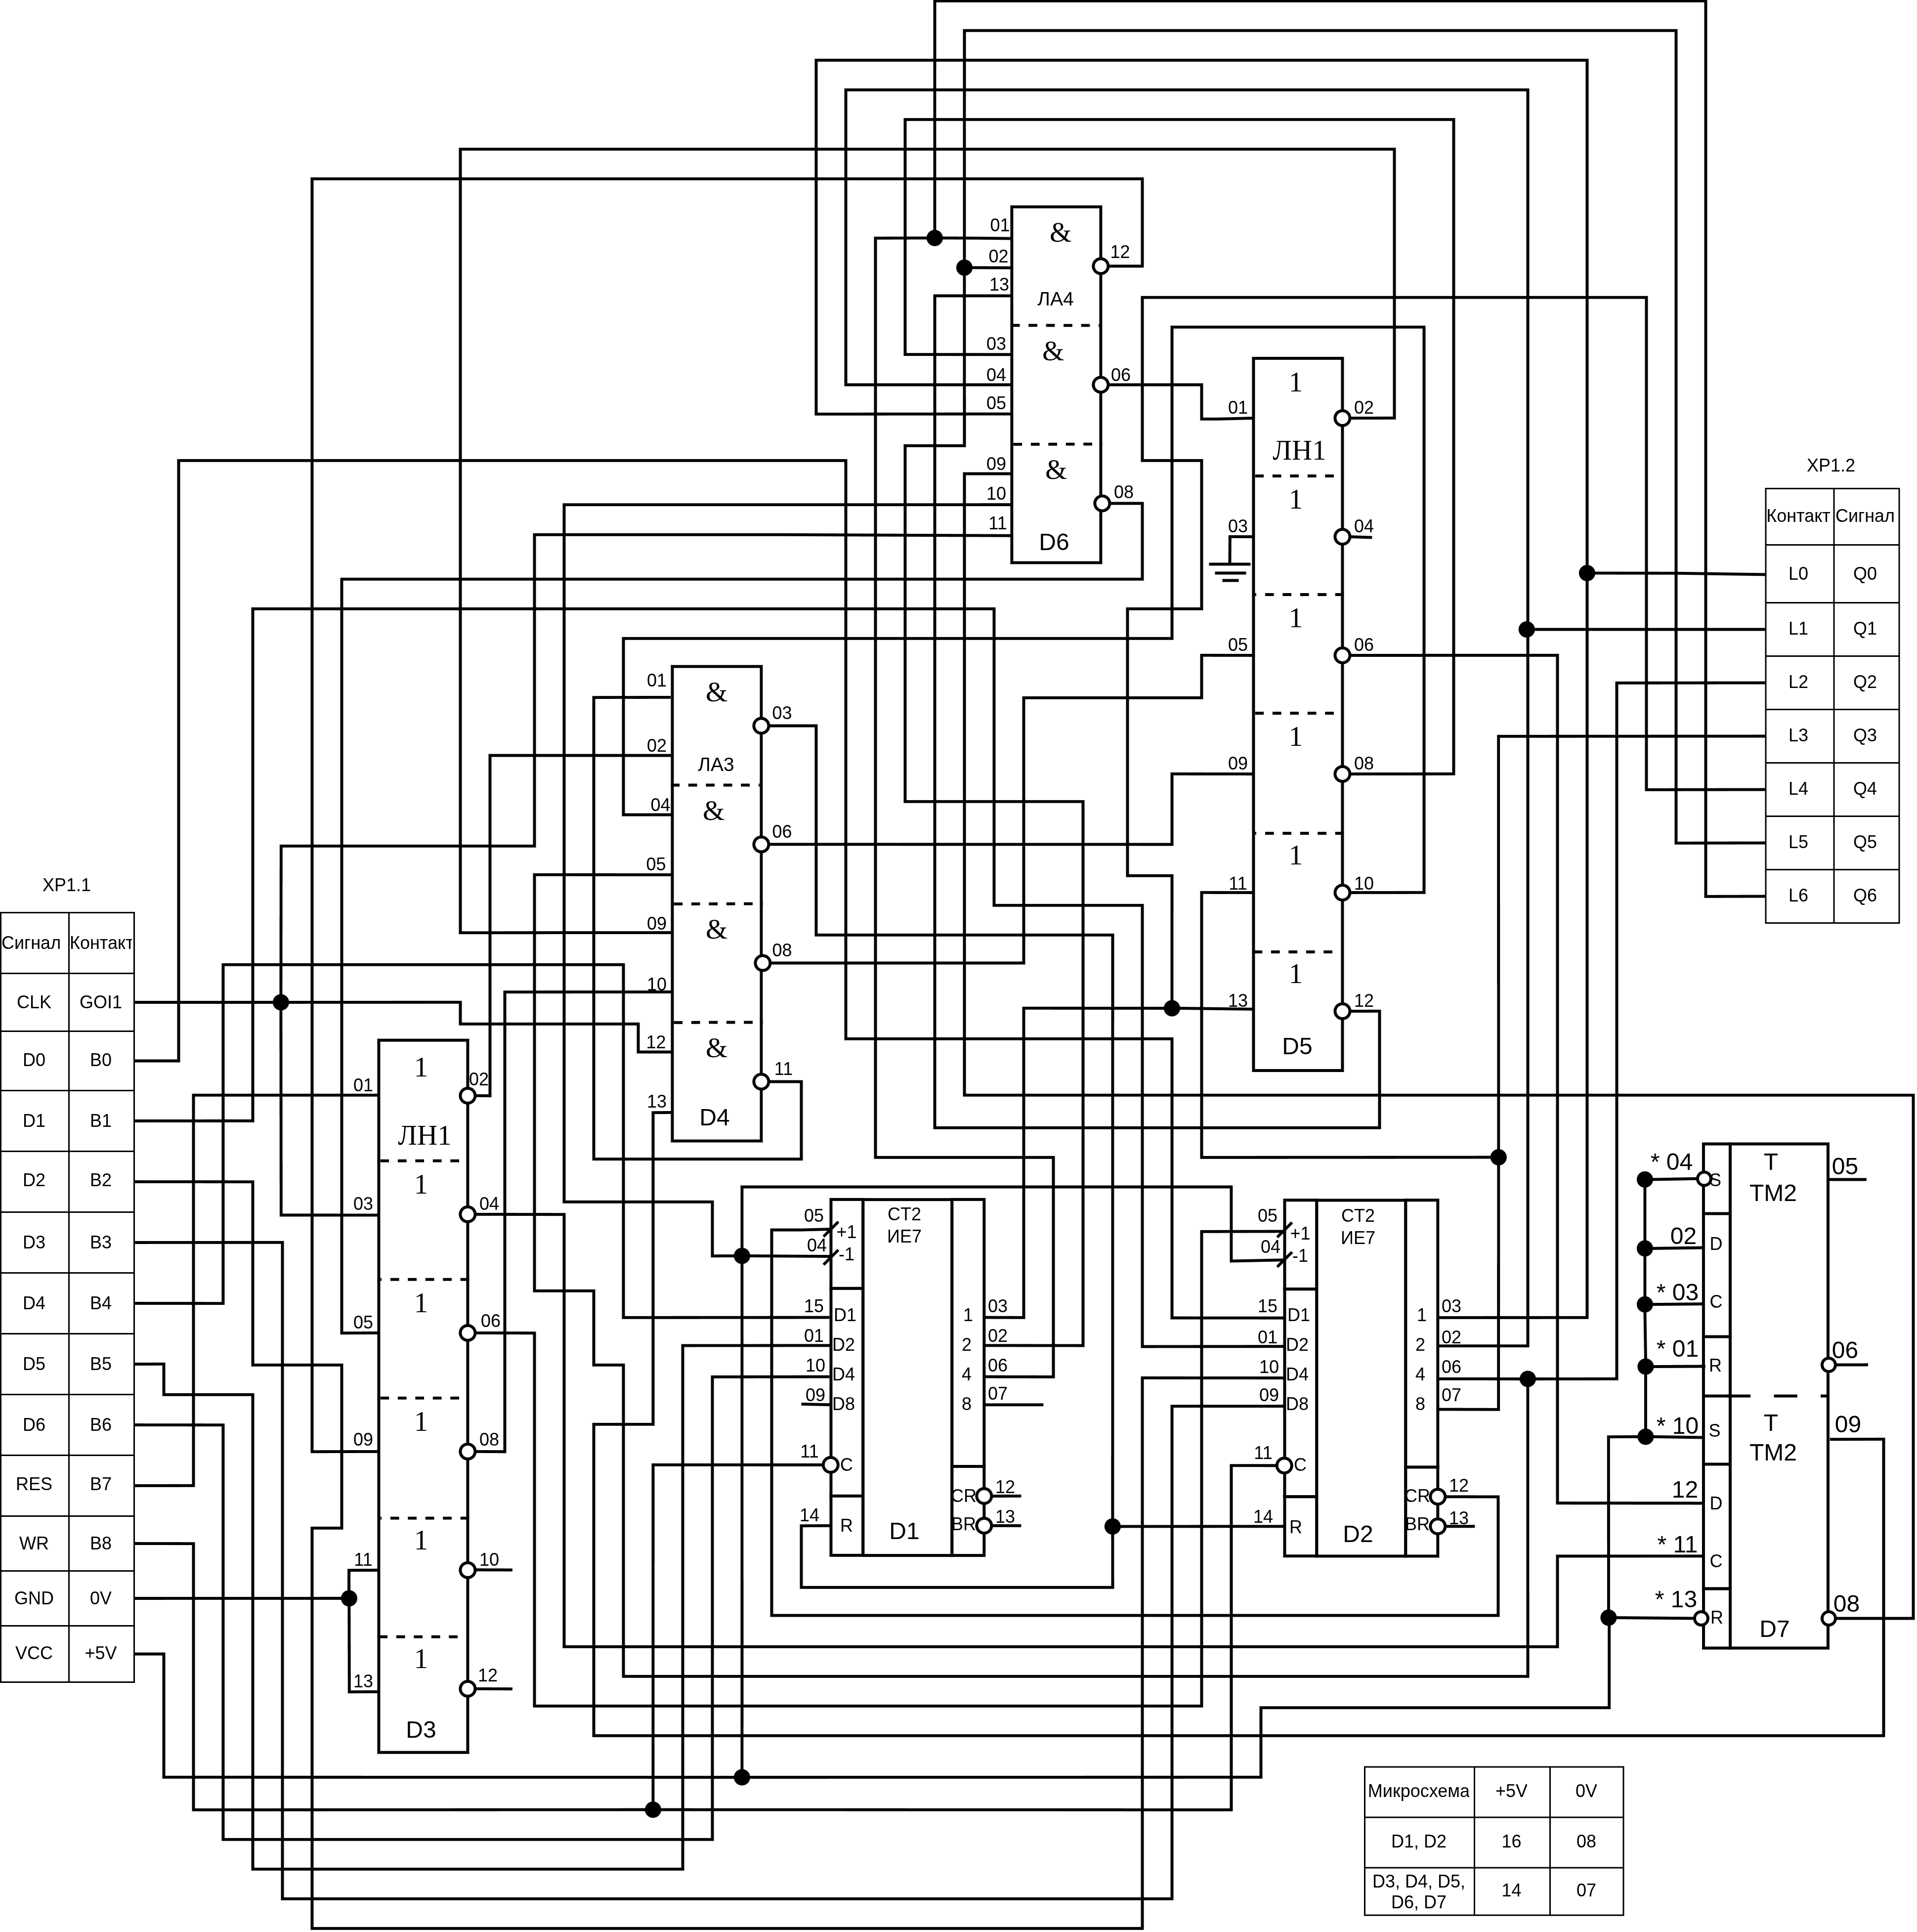
\includegraphics[width=0.95\textwidth]{pics/principle_diagram.png}
  \caption{Принципиальная электрическая схема счётчика с коэффициентом пересчёта 103}
\end{figure}

\section*{Вывод}
В ходе выполнения контрольной работы были освоены практические методы синтеза последовательностных схем с укороченным циклом работы. Спроектированный 7-битный счётчик с коэффициентом деления 103 на базе микросхем К155ИЕ7 и управляющего комбинационного автомата успешно решает задачу формирования произвольного периода счёта. Использование D-триггера К155ТМ2 в цепи сброса гарантирует надёжность функционирования системы и защищает её от ложных срабатываний, вызванных задержками распространения сигналов на логических вентилях.

\end{document}